% !TeX encoding = ISO-8859-1
\chapter{Management Summary}
\label{chap:managementsummary}

Die Linux Foundation hat mit dem Projekt Zephyr mit der Entwicklung eines
Echtzeit-Betriebssystems f�r das Internet der Dinge (IoT) begonnen.
Zephyr ist ein Open-Source-Betriebssystem mit dem Ziel, ein solides OS f�r IoT Ger�te
mit geringen Ressourcen bereitzustellen. Es nutzt eine echtzeitf�hige Kombination aus
Nano- und Microkernel.

Im Gegensatz zu einem Linux Kernel ben�tigt Zephyr nur zwischen 8 und 512 KByte an
Arbeitsspeicher. Aktuell werden folgende Plattformen unterst�tzt: x86, ARM und ARC
EM4.


\vspace{20mm}
\begin{figure}[h]
	\centering
	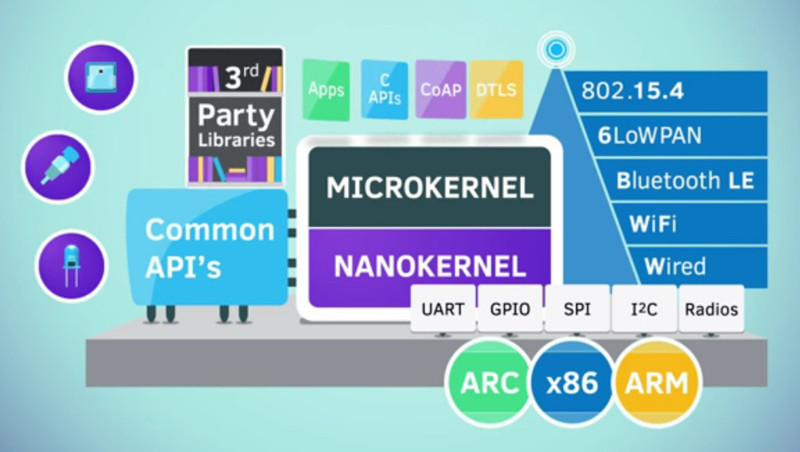
\includegraphics[width=0.7\linewidth]{bilder/zephyr_components.jpg}
	\caption{Komponente und �bersicht �ber das Zephyr RTOS}
	\label{fig:components}
\end{figure}
\vspace{7mm}
